In this related work section we will discuss a number of methods used for model checking timed automata. We will choose a method to extend our work on, and go more into detail on that method.

\subsection{Methods}
Already several model checkers for timed automata exist such as UPPAAL~\cite{UPPAAL}, KRONOS~\cite{kronos}, RABBIT~\cite{CAV03} and RED~\cite{crds}. We focus mainly on the UPPAAL tool as we use the same input format. Opaal~\cite{opaal}, the language module for LTSmin, uses the XML format that is created by the UPPAAL tools. This way we can use the UPPAAL user interface to create and adapt models. We also use the UPPAAL DBM library to represent zones. Several methods exist to represent the clock variables in a timed model. The most used methods are digitization and zones. 

Digitization approximates the continuous values of clocks by using discrete values~\cite{CHARME01}. This approach is however very sensitive to the granularity of the values used and the upper bound of the clock values. When fine granularity or large upper bounds are used, the memory usage will increase too much. An advantage of this approach is that basic model checking approaches can be used and no extra complexity due to zone calculations is added. The method however only works for closed timed automata, meaning that no strict comparisons on clocks can be made in the model. In ~\cite{nguyen2012discrete} a similar approach is proposed by using clock tick actions and removing clock variables altogether. 

The most established method to represent clock zones are DBMs~\cite{dbmorig, bengtsson2002clocks}. DBMs use a matrix structure that gives an lower and upper bound to each clock and to the difference between each pair of clocks. By this approach convex zones of clocks can be created. By using graph algorithms a normal form can be found quite efficiently. The downside of this approach is that only convex zones can be represented, when a state has multiple zones that are not a convex combination multiple DBMs are needed and thus increasing the memory usage. 

Several methods based on BDDs have been developed to represent zones. All of these are similar to DBMs in the sense that they use clock constraints to represent the zones. They use a BDD-like structure to represent the zones more efficiently. CDDs~\cite{BRICS19491} use single nodes for each variable and have disjoint intervals for that variable on the edges. This results in a node with a larger fanout and the upper and lower bound in a single node. DDDs~\cite{ddds, ddd-datastructure-99} use a constraint on each node that can either be true or false, when a constraint is false a next node will have another constraint on the same variable. This requires a fixed ordering based on the variables, values and operators. CRDs~\cite{crds} differ mainly from CDDs by using not disjoint intervals but possibly overlapping upper bounds for a variable pair on their edges. This diagram will have a larger fanout, like CDDs. They also use several normal forms for the diagrams which results in different performances. It is also shown that CRDs can be combined with BDDs into a single structure to fully symbolic represent state space. CMDs~\cite{5702245} combine CDDs, CRDs and DBMs into a single structure. This diagram type differs from the others by having multiple constraints per edge, resulting in a diagram with few nodes. CMDs do not have a normal form so only reduced forms are proposed. In ~\cite{7098276, 7184781} a method is proposed purely based on BDDs by translating the constraints directly into BDD nodes. This results in a unified structure for both the discrete variables and the clock constraints. The method is only a proof of concept and has not been implemented in a model checker and no performance results are known. In figure \ref{fig:examples} we have an example of all four BDD like structures representing the zone $2 < c_1 - c_2 < 4 \vee 7 \leq c_1 - c_2 \leq 8$.

\begin{figure}[b]
\begin{center}

	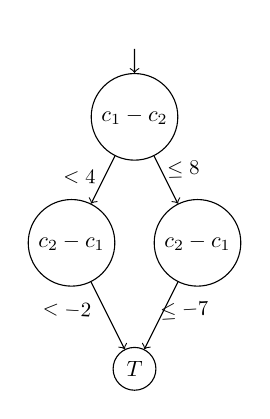
\begin{tikzpicture}[
		smallvertex/.style={circle,draw,scale=0.8}
		]
		\node[smallvertex](S0){$c_1 - c_2$};
		\node[smallvertex, draw = none, above of = S0, yshift = 0.25cm](S4){};
		\draw[->] (S4) --(S0) node [midway, above, sloped, scale=0.75,
		rotate=295, xshift =-0.4 cm, yshift = -0.2cm]{};
		\node[smallvertex, below of = S0, yshift = -1 cm, xshift = -1 cm](S1){$c_2 - c_1$};
		\node[smallvertex, below of = S0, yshift = -1 cm, xshift = 1  cm](S2){$c_2 - c_1$};
		\draw[->] (S0) --(S1) node [midway, above, sloped, scale=0.75,
		rotate=295, xshift =-0.4 cm, yshift = -0.2cm]{$<4$};
		\draw[->] (S0) --(S2) node [midway, above, sloped, scale=0.75,
		rotate=65, xshift =0.3 cm, yshift = -0.1cm]{$\leq 8$};
		\node[smallvertex, below of = S0, yshift = -3cm](S3){$T$};
		\draw[->] (S1) --(S3) node [midway, above, sloped, scale=0.75,
		rotate=60, xshift =-0.7 cm, yshift = -0.2cm]{$<-2$};
		\draw[->] (S2) --(S3) node [midway, above, sloped, scale=0.75,
		rotate=300, xshift =0.4 cm, yshift = -0.2cm]{$\leq-7$};
	\end{tikzpicture}
	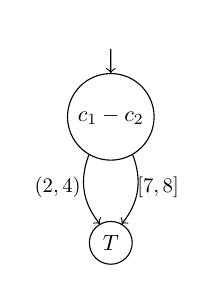
\begin{tikzpicture}[
		smallvertex/.style={circle,draw,scale=0.8}
		]
			
		\node[smallvertex](S0){$c_1 - c_2$};
	    \node[smallvertex, draw = none, above of = S0, yshift = 0.25cm](S4){};
		\draw[->] (S4) --(S0) node [midway, above, sloped, scale=0.75,
		rotate=295, xshift =-0.4 cm, yshift = -0.2cm]{};
		\node[smallvertex, below of = S0, yshift = -1cm](S3){$T$};
		\draw[->] (S0) edge [bend left](S3) node [midway, above, sloped, scale=0.75,
		rotate=0, xshift =-0.9 cm, yshift = -1.5cm]{$(2,4)$};
		\draw[->] (S0) edge [bend right](S3) node [midway, above, sloped, scale=0.75,
		rotate=0, xshift =0.8 cm, yshift = -1.5cm]{$[7,8]$};
	\end{tikzpicture}	
	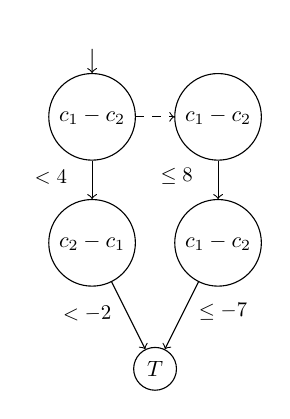
\begin{tikzpicture}[
		smallvertex/.style={circle,draw,scale=0.8}
		]
			
		\node[smallvertex](S0){$c_1 - c_2$};
		\node[smallvertex, draw = none, above of = S0, yshift = 0.25cm](S5){};
		\draw[->] (S5) --(S0) node [midway, above, sloped, scale=0.75,
		rotate=295, xshift =-0.4 cm, yshift = -0.2cm]{};
		\node[smallvertex, right of = S0, xshift = 1cm](S1){$c_1 - c_2$};
		\draw[dashed,->] (S0) --(S1) node [midway, above, sloped, scale=0.75,
		rotate=0, xshift =-0.7 cm, yshift = -0.2cm]{};
		\node[smallvertex, below of = S0, yshift = -1cm](S2){$c_2 - c_1$};
		\draw[->] (S0) --(S2) node [midway, above, sloped, scale=0.75,
		rotate=90, xshift =-0.7 cm, yshift = -0.2cm]{$< 4$};
		\node[smallvertex, below of = S1, yshift = -1cm](S3){$c_1 - c_2$};
		\draw[->] (S1) --(S3) node [midway, above, sloped, scale=0.75,
		rotate=90, xshift =-0.7 cm, yshift = -0.2cm]{$\leq 8$};
		\node[smallvertex, below of = S0, xshift = 1cm, yshift = -3cm](S4){$T$};
		\draw[->] (S2) --(S4) node [midway, above, sloped, scale=0.75,
		rotate=65, xshift =-0.7 cm, yshift = -0.2cm]{$<-2$};
		\draw[->] (S3) --(S4) node [midway, above, sloped, scale=0.75,
		rotate=297, xshift =0.7 cm, yshift = -0.2cm]{$\leq-7$};
	\end{tikzpicture}
	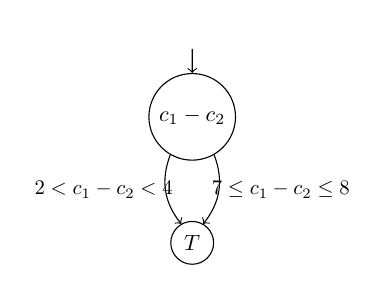
\begin{tikzpicture}[
		smallvertex/.style={circle,draw,scale=0.8}
		]
			
		\node[smallvertex](S0){$c_1 - c_2$};
		\node[smallvertex, draw = none, above of = S0, yshift = 0.25cm](S4){};
		\draw[->] (S4) --(S0) node [midway, above, sloped, scale=0.75,
		rotate=295, xshift =-0.4 cm, yshift = -0.2cm]{};
		\node[smallvertex, below of = S0, yshift = -1cm](S3){$T$};
		\draw[->] (S0) edge [bend left](S3) node [midway, above, sloped, scale=0.75,
		rotate=0, xshift =-1.5 cm, yshift = -1.5cm]{$2<c_1-c_2<4$};
		\draw[->] (S0) edge [bend right](S3) node [midway, above, sloped, scale=0.75,
		rotate=0, xshift =1.5 cm, yshift = -1.5cm]{$7\leq c_1-c_2\leq8$};
	\end{tikzpicture}	
	
\end{center}
\caption{A CRD, CDD, DDD and CMD representation}
\label{fig:examples}
\end{figure}

\begin{table}[]
\centering
\caption{Comparing Diagrams}
\label{table:diagrams}
\begin{tabular}{|l|l|l|}
\hline
Type                                                   & Pro                                                                                                                                                                                                                             & Con                                                                                                                                                                                                                                                          \\ \hline
DBM                                                    & \begin{tabular}[c]{@{}l@{}}Canonical form for convex zones\\ Existing library\\ Inclusion check\end{tabular}                                                                                                                    & \begin{tabular}[c]{@{}l@{}}Concave zones need multiple DBMs\\ Not memory efficient\end{tabular}                                                                                                                                                              \\ \hline
DDD                                                    & \begin{tabular}[c]{@{}l@{}}Structure like LDD\\ Re-ordering of variables possible\\ Apply same efficiency as BDDs\\ Boolean variables also in DDD\end{tabular}                                                                  & \begin{tabular}[c]{@{}l@{}}Canonicity hard to obtain\\ No on the fly canonicity\\ Expensive normal form computation\\ Only time performance tested\\ Only reduction algorithms\end{tabular}                                                                  \\ \hline
CDD                                                    & \begin{tabular}[c]{@{}l@{}}Structure like MDD\\ Inclusion check\\ (intersection of complement)\end{tabular}                                                                                                                     & \begin{tabular}[c]{@{}l@{}}No algorithm to get normal form\\ Only high level algorithms given\\ Methods don't maintain disjointness\\ Expensive normal form computation\\ No implementation results available\\ Disjointness memory inefficient\end{tabular} \\ \hline
CRD                                                    & \begin{tabular}[c]{@{}l@{}}Combination with BDD possible\\ Variable reordering shows advantage\\ Library available\\ Some benchmarks exp better than CDD\\ Extensive benchmarks\\ Good performance backwards reach\end{tabular} & \begin{tabular}[c]{@{}l@{}}3 possible canonical forms\\ No algorithms in paper\\ Some benchmarks linear worse than CDD\end{tabular}                                                                                                                          \\ \hline
CMD                                                    & Benchmarks against RED and UPPAAL                                                                                                                                                                                               & \begin{tabular}[c]{@{}l@{}}Results differ per case\\ Needs translation from vector to edges\\ Two reduced forms\end{tabular}                                                                                                                                 \\ \hline
\begin{tabular}[c]{@{}l@{}}BDD\\ discrete\end{tabular} & \begin{tabular}[c]{@{}l@{}}Using existing BDD packages\\ Good performance for small clock values\end{tabular}                                                                                                                   & \begin{tabular}[c]{@{}l@{}}Performance decreases fast for large values\\ Not possible with current opaal PINS\\ Introducing additional 'tick' actions\\ Only for closed timed automata\end{tabular}                                                          \\ \hline
\begin{tabular}[c]{@{}l@{}}BDD\\ zones\end{tabular}    & \begin{tabular}[c]{@{}l@{}}Using existing BDD packages\\ All variable reorderings possible\\ Only need direct translation DBM to\\ state vector\\ Easy to implement\end{tabular}                                                & \begin{tabular}[c]{@{}l@{}}Losing zone containment\\ No implementation results\end{tabular}                                                                                                                                                                  \\ \hline
\end{tabular}
\end{table}

A known difficulty in BDDs is the variable ordering. A bad ordering can lead to a BDD exponential in size where a good ordering can sometimes lead to a significant smaller diagram. Of the zone diagrams named above only for CRDs experiments with different orderings have been conducted, the other researches assume a given ordering on the variables and the ordering of the values is fixed. The CRD case shows that full interleaving and having related variables close to each other in the ordering is preferable and gives the best results, both on speed and memory. This is the same result as expected with BDDs, this suggests that similar orderings should be used with these techniques. In table \ref{table:diagrams} we compare the different types of diagrams we discussed above.

\begin{figure}[t] 
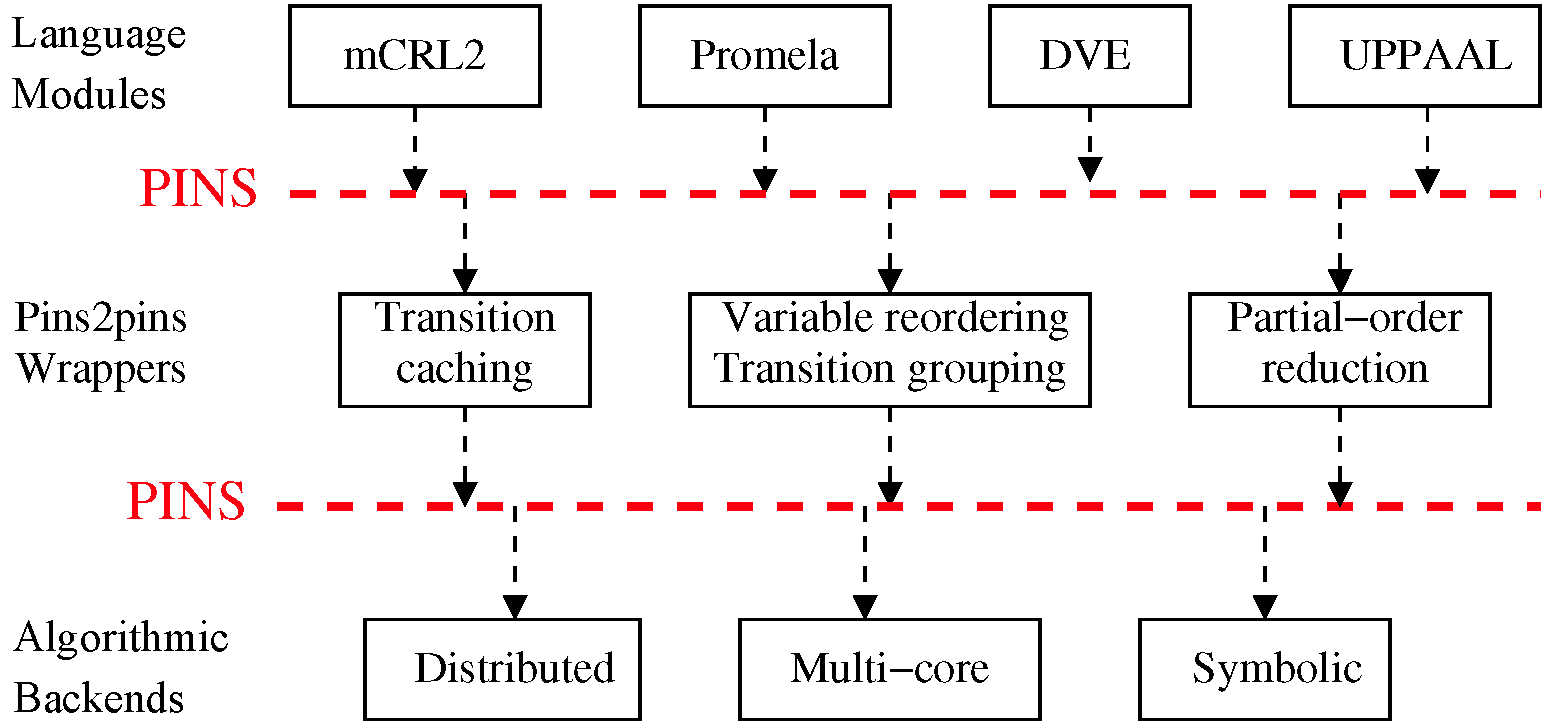
\includegraphics[width=\textwidth]{pins_modern}
\caption{Modular structure of LTSmin}
\label{fig:pins_modern}
\end{figure}

\subsection{LTSmin}
LTSmin~\cite{eemcs18152,ltsmin-mc:nmf2011} is a language independent model checker. It is built in a modular way such that new languages can be added by a PINS (Partitioned Next-State Interface) interface without too much effort, and new algorithms can be added easily. LTSmin offers four different algorithmic back ends for model analysis: symbolic, multi-core, sequential and distributed. All of these back ends support different types of reduction and model checking. Several language modules have already been built for LTSmin such as mCRL2, Promela, DVE and UPPAAL. The modular structure of LTSmin is shown in figure \ref{fig:pins_modern}. The PINS is the core of LTSmin. This interface abstracts as much as possible from the model without losing the structure. It represents states as fixed length integer arrays. The main function of the interface is a (partitioned) next state function which returns the successor states. With these functions a state space can be generated on the fly. With the use of dependency matrices event locality can be determined statically~\cite{rwcmatrices}. Using these matrices, more efficient symbolic algorithms can be used, the number of next-state calls can be reduced, efficient variable reorderings can be used, and transition caching can be used. In the current UPPAAL PINS the next-state function is not partitioned and therefore no meaningful dependency matrix is created, and none of these algorithms can be used.

\subsection{Difference Decision Diagrams}

We have discussed several symbolic approaches for representing zones. All of these approaches have benefits and downsides over each other. We chose to develop one of these approaches in LTSmin. We wanted a diagram that can store both discrete states and zones, this can either be done in the diagram, or in a combination of the diagram and BDD or LDD nodes. Also a subsumption check on the diagram should be possible. We chose from the four zone representing diagrams discussed earlier. The CDD approach was not chosen due to the memory inefficient disjoint intervals and their algorithms not maintaining these intervals, the CMD approach is too similar to DBMs, on which we already have an approach. The choice between CRD and DDD was between two quite similar diagrams. We have decided to continue on the DDD. It is a diagram form that is closely related to LDDs, for which we already have a library, and it is also quite compatible to the current PINS structure and its' next state function. The method still has some loose ends that need research, mostly on the algorithms and efficiently creating a canonical form. No results on the memory usage are available, which is normally the greatest benefit of a symbolic approach, so also on the results side we extend the current research. So DDDs are a diagram type that seems to fit well in the current structure we have, but there is still room for some more research. First we give the definition of a DDD.

\begin{mydef}[Difference Decision Diagram~\cite{ddds}]
\label{def:DDD}
A difference decision diagram (DDD) is a directed acyclic graph $(V,E)$. The vertex set $V$ contains two terminals $0$ and $1$ with out-degree zero, and a set of non-terminal vertices with out-degree two and the following attributes.
\\\\
\begin{tabular}{lll}
Attribute                & Type                      & Description                                           \\\hline
pos(v), neg(v)           & \textbf{Var}              & Positive variable $x_i$, and negative variable $x_j$. \\
op(v)                    & \{\textless, $\leq\}$     & Operator \textless or $\leq$.                         \\
const(v)                 & $\mathbb{D}$              & Constant c.                                           \\
high(v), low(v)          & $V$                       & High-branch h, and low-branch l.                   
\end{tabular}
\captionof*{table}{}  
The set E contains the edges $(v,low(v))$ and $(v, high(v))$, where $v \in V$ is a non-terminal vertex.
\end{mydef}

In ~\cite{ddds} a canonical form for DDDs is discussed, also called a fully reduced DDD. Only definitions are given here, no algorithms to reach this form. It is stated that it is difficult to reach this fully reduced form. It is not clear if they managed to make their apply function in such a way that it maintains canonicity. To reach canonicity, local reductions and ordering are a first step, but it is not enough due to dependencies among the constraints. For BDDs the local reductions and ordering are sufficient to reach a canonical form. First we give some notational shorthands and then we define an ordering and local reductions on DDDs.
%
\begin{center}
\begin{tabular}{lll}
$var(v)$   & $=$ & $(pos(v),neg(v))$   \\
$bound(v)$ & $=$ & $(const(v),op(v))$  \\
$cstr(v)$  & $=$ & $(var(v),bound(v))$
\end{tabular}
\end{center}

\begin{mydef}[Ordered DDD~\cite{ddds}]
\label{def:ODDD}
An ordered DDD (ODDD) is a DDD where each non-terminal vertex $v$ satisfies:
\begin{enumerate}
  \item $neg(v) \prec pos(v)$,
  \item $var(v) \prec var(high(v))$,
  \item $var(v) \prec var(low(v))$ or \\ $var(v) = var(low(v))$ and $bound(v) \prec bound(low(v))$.
\end{enumerate}
\end{mydef}

After ordering a DDD some local reductions can be defined to reduce the size of a DDD.

\begin{mydef}[Locally Reduced DDD~\cite{ddds}]
A locally reduced DDD ($R_LDDD$) is an ODDD satisfying, for all non-terminals u and v:
\begin{enumerate}
  \item $\mathbb{D} = \mathbb{Z}$ implies $op(v) = '\leq'$,
  \item $(cstr(u),high(u),low(u)) = (cstr(v),high(v),low(v))$ implies $u = v$,
  \item $low(v) \neq high(v)$,
  \item $var(v) = var(low(v))$ implies $high(v) \neq high(low(v))$.
\end{enumerate}
\end{mydef}

These reductions are not enough to reach a canonical form. Here we define the other reductions and methods needed to reach a canonical form.

\begin{mydef}[Path-reduced DDD~\cite{ddds}]
A path-reduced DDD ($R_PDDD$) is a locally reduced DDD where all paths are feasible.
\end{mydef}

\begin{mydef}[Tightness~\cite{ddds}]
A dominating constraint $\alpha = x_i - x_j \lesssim c$ is tight in a feasible path $[p] = [p_1] \wedge \alpha \wedge [p_2]$ if for all tighter constraints $(c', \lesssim') < (c,\lesssim),$ the systems $[p_1] \wedge (x_i - x_j \lesssim' c') \wedge [p_2]$ and $[p]$ have different solutions. A path $p$ is tight if it is feasible and all dominating constraints on it are tight. An $R_LDDD u$ is tight if all paths from $u$ are tight. 
\end{mydef}

\begin{mydef}[Saturation~\cite{ddds}]
A tight path $p$ from an $R_PDDD$ is saturated if for all constraints $\alpha$ not on $p$, if $\alpha$ is added to $p$ either (1) $\alpha$ is not dominating and tight, or (2) the constraint system $[p_1] \wedge \neg\alpha$ is infeasible when $[p]$ is written $[p] = [p_1] \wedge [p_2]$ with all constraints on $p_1$ smaller than $\alpha$ with respect to $\prec$ and all constraints on $p_2$ larger than $\alpha$. An $R_PDDD$ $u$ is saturated if all paths from $u$ are saturated.
\end{mydef}

\begin{mydef}[Disjunctive vertex~\cite{ddds}]
Let $p$ be a path leading to the vertex $u$ in a DDD, and assume $\alpha = cstr(u), h = high(u),$ and $l = low(u)$. Then $u$ is disjunctive in $p$ if $[p] \wedge (\alpha \rightarrow h,l)$ and $[p] \wedge (h \vee l)$ have the same set of solutions.
\end{mydef}

All of these definitions together lead to the following definition of a fully reduced DDD.
% 
\begin{mydef}[Fully reduced DDD~\cite{ddds}]
\label{def:RFDDD}
An $R_pDDD$ u is a fully-reduced DDD ($R_FDDD$) if it is tight, saturated and has no disjunctive vertices.
\end{mydef}

DDDs are also used to represent the discrete variables in automata. This is done by translating the variable into a difference constraint. For example $x_1 = 3$ will be translated into $x_1 - 0 \leq 3 \wedge 0 - x_1 \leq -3$, thus resulting into a DDD with two nodes. 

So far we only found the results of two benchmark tests of DDDs, Milner's scheduler and Fischer's protocol~\cite{Møller200253}. Here the DDD approach has been compared with KRONOS and UPPAAL which were both slower than the DDD implementation. The results of these benchmarks show no memory usage.  